This chapter is my notes from a Udemy Course called \textbf{Deep Reinforcement Learning 2.0}. During the course I will see theory notions but implementations of some AI that keeps learn. I will face Q-Learning and other cool stuff.

The structure of the course will be:
\begin{itemize}
\item Extra theory
\item Foundamentals
\item Twin Delayed DDPG - Theory
\item Twin Delayed DDPG - Implementation
\end{itemize}

\section{Resources}
\url{https://arxiv.org/pdf/1802.09477.pdf}. It is the paper that we will discuss dring the course


\section{Extra theory: basic knowledge}

In this section we will see what is reinforcement learning, Bellman equation, Markov decision process, plans,  living penalty, q-learning, temporal difference.

\subsection{Reinforcement Learning}
 The main ingredients of a RL systems are:
 \begin{itemize}
 \item Agent: the AI that has to fulfill  a task by taking actions
 \item Environment: the place where Agent lives
 \item Action and rewards: mechanism that make Agent do thing and discriminate if it is right or not. Action are hard coupled with time.. a correct action in a wrong time leads a bad rewards.
 \end{itemize}
 
 Training AI is like training a dog, if it does right it get a reward otherwise nothing.
 
 \begin{figure}
    \centering
    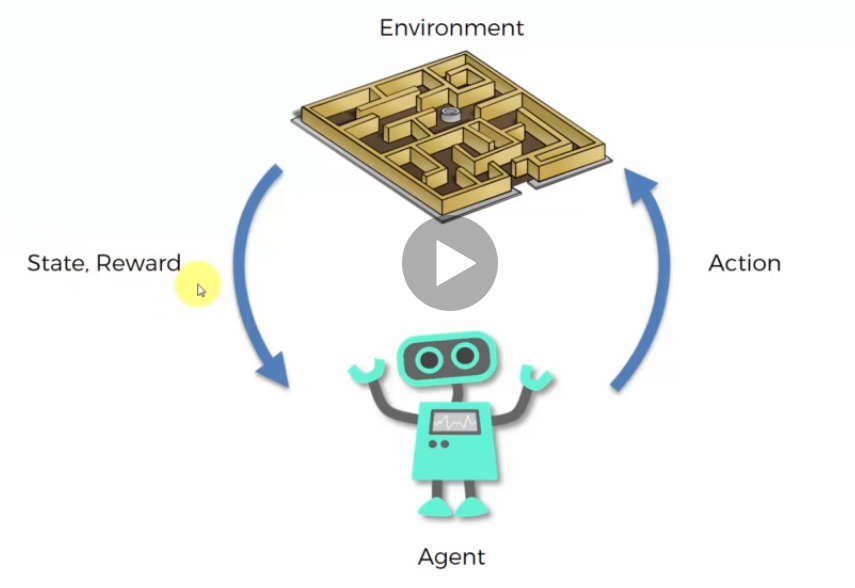
\includegraphics[scale=0.65]{img/reinforcementlearning01.png}
    \caption{Overview of Reinforcement Learning system}
    \label{img:RL-System}
\end{figure}

RL create RL agents that differs from Pre-Programmed Agents by the knowledge they have inside before start learning. The PPAgents have a series of rule that describe all actions they can do, in which case etc etc... while RL has to figure out those rule, his own behavior.

\subsection{BellMan Equation}

Notions:
\begin{itemize}
 \item $s$ the state of the agent
 \item $a$ action that agent can make
 \item $R$ reward agent gets for entering in a State
 \item $y$ Discount. 
 \end{itemize} 
 
  \begin{figure}
    \centering
    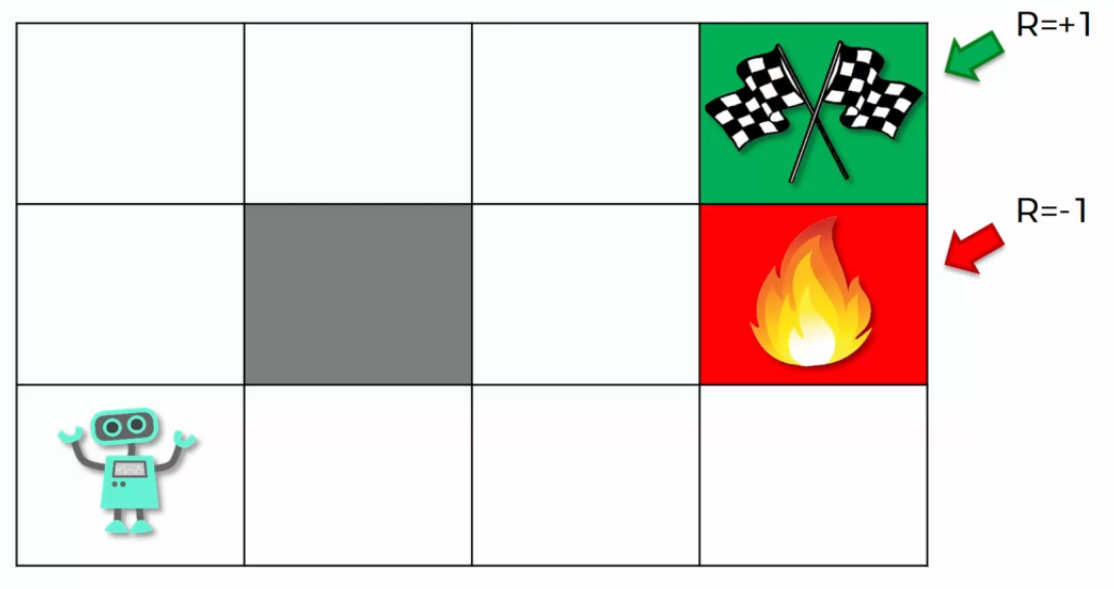
\includegraphics[scale=0.35]{img/rl-maze.png}
    \caption{RL - Maze task}
    \label{img:RL-Maze}
\end{figure}

 Before start let's define a task. We have an agent (the robot) in a maze composed by a grid with three different kinds of cells:
 \begin{itemize}
 \item Empy: the withe cell where agent is free to go
 \item Grey: the wall, agent cant cross this cell
 \item Red: The fire, agent can go there but it loses
 \item Green: the target, agent can go there and it wins
 \end{itemize}
 You can see this amazing maze in the picture \ref{img:RL-Maze}
 The agent can do 4 actions:
 \begin{itemize}
 \item Go Up
 \item Go Down
 \item Go Right
 \item Go Left
 \end{itemize}

\textbf{Basic Idea Of Bellman equation}. When agent goes to the green cell it gets a +1 rewards. It likes rewards, it is addicted, it cant live without so it think: "how i get the reward?" in order to be able to get it each time. So it learns that from the previous cell (3,3) it has to just move right (4,3) and he get the +1. Now each time it goes in (3,3) he knows how to get reward. He is happy but he could be more happy, more addicted. He start to think: "how i get here in the (3,3)" in order to be able to get this cell every time. So it learn for example that it can reach this cell from (3,2). Then it ask the same until it has learned a path from the start point to the green cell. Now it is really happy. 

\textbf{The bellman equation}. This is the bellman equation:
\begin{equation}
V(s) = max_a(R(s,a) + yV(s'))
\end{equation}
This equation gives a value $V$ to a State $s$ reached by the agent. The value is based on the best action it can take from that state. Let dig into it. We know agent in a state can take actions $a$, in our case it can chose between 4 actions each of them leads the action is a new state $s'$. Each action, took in a state has a reward for example if agent is in (3,3) and it goes right it get +1 as reward, if it is in (3,2) and it goes right it get -1 as reward because it ends in the fire. So each action, according to the current state, leads to different rewards $R(a,s)$. In the bellman equation we select the action that give the maximum value. So we cycle on all possible action computing the reward $R(s,a)$ and we select the action that brings agent to the greatest reward. We also consider the value of the reached state. Take an action brings agent from $s$ to $s'$ so the value of $s'$ must be taken in account $yV(s')$. So for each action we compute the reward $R(s,a)$ plus the value of the reached state $yV(s')$ and we select the action that gives the agent the greatest value because we want agent be optimal, so we can consider just best solutions.

\textbf{Let's do some example}
Let's compute the $V(s)$ of the (3,3) using a $y = 0.9$.
$V((3,3)) = R((3,3), goRight) + yV((3,4))$. We already know the best action because it is the only action that leads agent to the target (3,4). So considering this action we compute the value.

$V((3,3)) = 1 + y0$ V(3,4) is zero cause it is the target cell and we don't need it to have a value
So $V((3,3)) = 1$

We can repeat this for the V(2,3), we know the best action is go right so $V(2,3) = 0 + 0.9 * 1 = 0.9$. We can repeat the it for each cell.

\begin{figure}
    \centering
    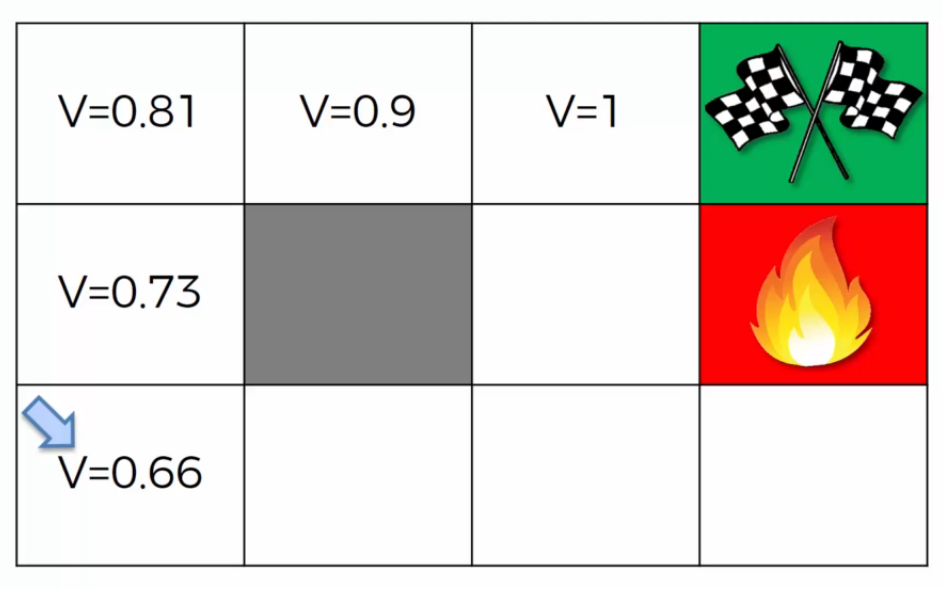
\includegraphics[scale=0.35]{img/rl-maze-be.png}
    \caption{RL - Maze task with values from bellman equation}
    \label{img:RL-Maze}
\end{figure}

It easy to see that value decreases according to the distance to the target cell (4,3).

\subsection{Stochastic variable... OMG}
Untill now we speak about the maze a a very kind one. U want to go up, then u go up with 100\% possibility. But this is not how real life, out there, works. Let's add some randomness, let's create a stochastic maze where the action is a stochastic process. For example in cell (2,3) ground is broken so if u want to go up you have: 
\begin{itemize}
\item 80\% of probability to go up
\item 10\% of fall down
\item 10\% of fall in the cell with the hell's fire and die.
\end{itemize}

This is a \textbf{Markov Process} because the state $s'$ is expressed just according to the current state and not the previous decision of the agent. (Check the chapter about Markov Process).

That is how real work works. Our robot, that is addicted wish to get to the cell (3,3) because it perfectly know how to reach is drug from there. So from (3,2) decide to go up but it risk to fail and worsening his position. So the value of this cell must decrease.

Let's define the new Bellman Equation considering the Markov Decision Process:
\begin{equation}
V(s) = max_a(R(s,a) + y \sum_{n} P(s,a,s'_n)V(s'_n))
\end{equation}
Let's explain that, now agent can end in different states $s'_1 s'_2 ... s'_n$ and it can end there with a certain probability. Let's define P() as a function that gives to us this probability:
$P(s,a,s'_n)$ gives to us the probability from $s$ to reach $s'_n$ by action $a$. For each possible state $s'_n$ we need to compute this probability and multiply it with the value of that state and sum all values obtained.

Let's do an example. Let's compute the value of (3,2) considering the hard ground.
$V((3,2)) = 0 + 0.9 * ((0.8 * 1) + (0.1 * 0.73) + (0.1 * -1)) = 0.6957$

\begin{figure}
    \centering
    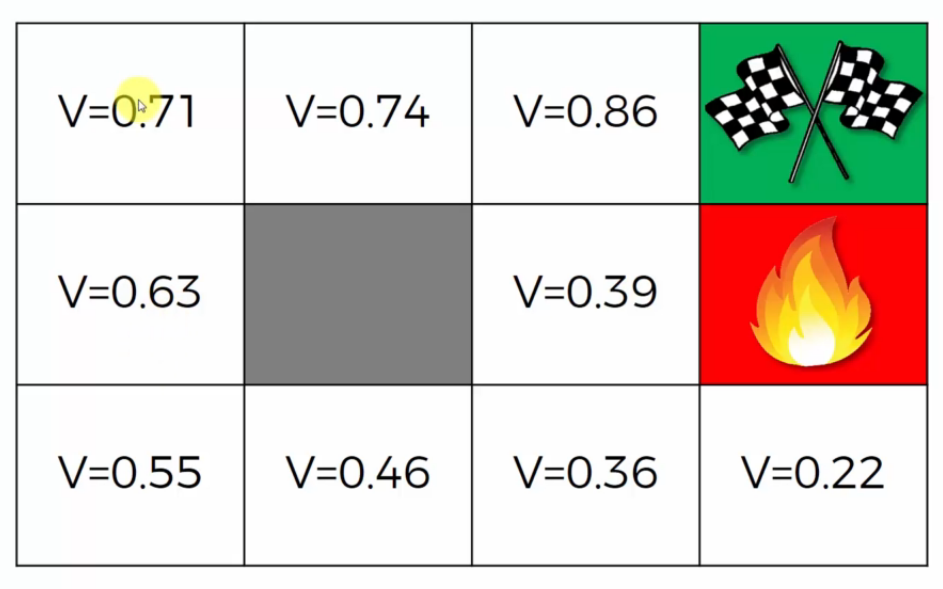
\includegraphics[scale=0.35]{img/rl-maze-stoch.png}
    \caption{RL - Maze task with all values changed because in each cell there is a probability to fall in two wrong cells}
    \label{img:RL-Maze-stoch}
\end{figure}

From pics \ref{img:RL-Maze-stoch} it's possbile to see the new cell values considering the probability to end in the wrong cells (80\%, 10\%, 10\%). That is why the agent in the cell (3,2) wont try to go up because he know that he have 10\% of probability to end in the fire an die. But it is more convenient for him to try to go in the wall an stay in the cell (3,2) but have a 20\% of probability to fall in a better cell without risk to end in the fire. It's possible to see it in the picture \ref{img:RL-Maze-plan}.

\begin{figure}
    \centering
    \includegraphics[scale=0.35]{img/rl-maze-plan.png}
    \caption{RL - Maze task with all values changed because in each cell there is a probability to fall in two wrong cells. We can see the actions that agent will try to take in each cell}
    \label{img:RL-Maze-plan}
\end{figure}

\subsection{Rewarding}

In our maze, by now, agent get two rewards the +1 if it arrives in the (4,3) cell (the green) or -1 if it ends in the fire. But what takes the agent away from waste time? Maybe it wants to walk a bit before get the reward? But we want agent be more addicted possible, we want it suffering the pain of hell if it doesn't get fast his drug!! Let's introduce \textbf{The Living Penalty}, a negative reward that it gets each time it take and actions. More action it takes more penalty if collects. Using this it select different action, for example it stops to try to go in the wall, has it does without penalty. You can see this differences in the picture \ref{img:RL-Maze-LP} 

\begin{figure}
    \centering
    \includegraphics[scale=0.35]{img/rl-maze-LP.png}
    \caption{RL - Actions for the maze with different Living Penalty}
    \label{img:RL-Maze-LP}
\end{figure}

\subsection{Q-Learning}
By now, using bellman equation, the best action is chosen by knowing the value of a state and selecting the action that brings agent it that state. In Q-Learning approach the idea is to evaluate directly the action using a \textit{Quality function} to measure the quality of an action $Q(s, a)$ where $s$ is the state of the agent  and $a$ is the action.
The $Q(s,a)$ equation come from this equation:
\begin{equation}
Q(s,a) = R(s,a) + y \sum_{n} P(s,a,s'_n)V(s'_n)
\end{equation}

As we can see it is identical to the final piece of bellman equation. But we still have $V(s)$ in our equation and we don't want it because it focuses on value of state and we want focus on value of possible action:

\begin{equation}
Q(s,a) = R(s,a) + y \sum_{n} P(s,a,s'_n) max_{a'}Q(s'_n, a')
\end{equation}